
\documentclass[12pt]{article}
\usepackage{amssymb, amsmath, amsfonts, bm, graphicx, geometry}
\usepackage{tabularx, booktabs, float, enumitem, multicol, mathtools}
\usepackage{parskip} % Auto-manages paragraph spacing and removes indentations
\usepackage{siunitx}  % Eases typesetting of numbers and units
\usepackage[hidelinks]{hyperref}
\usepackage{soul}
\usepackage{mathrsfs}
\usepackage{tikz}
\usetikzlibrary{arrows.meta, positioning, calc}

\geometry{margin=1in}

\begin{document}

\begin{center}
    \Large\textbf{Closed-Loop Feedback Control System}
\end{center}

\begin{figure}[H]
    \centering
    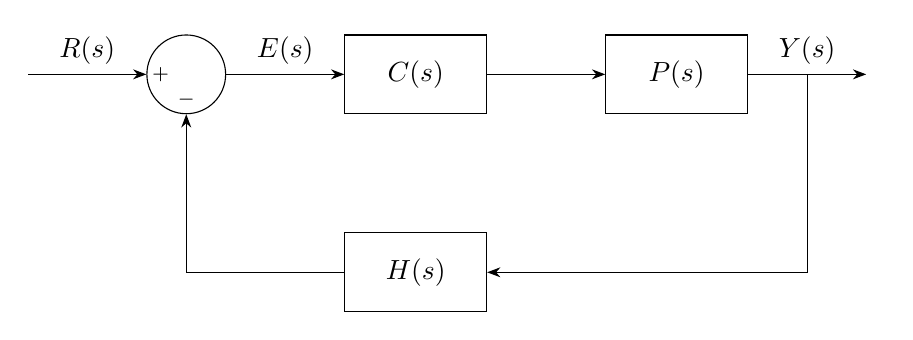
\begin{tikzpicture}[
        >=Stealth,
        block/.style={
            draw,
            rectangle,
            minimum width=1.8cm,
            minimum height=1cm
        },
        sum/.style={
            draw,
            circle,
            minimum size=1cm,
            inner sep=0pt
        },
        node distance=1.5cm
    ]

        % Nodes
        \node[sum] (sum) {};
        \node[block, right=1.5cm of sum] (controller) {$C(s)$};
        \node[block, right=1.5cm of controller] (plant) {$P(s)$};
        \node[right=1.5cm of plant] (output) {};
        \node[block, below=1.5cm of controller] (feedback) {$H(s)$};

        % Forward path
        \draw[->] ([xshift=-1.5cm]sum.west)
            -- node[above] {$R(s)$} (sum.west);

        \draw[->] (sum.east)
            -- node[above] {$E(s)$} (controller.west);

        \draw[->] (controller.east)
            -- (plant.west);

        \draw[->] (plant.east)
            -- node[above] {$Y(s)$} (output);

        % Feedback path
        \draw[->] ($(plant.east)+(0.75cm,0)$)
            |- (feedback.east);

        \draw[->] (feedback.west)
            -| (sum.south);

      % Summing junction signs
\node at ($(sum.west)+(0.18cm,0)$) {\scriptsize $+$};
\node at ($(sum.south)+(0,0.18cm)$) {\scriptsize $-$};

    \end{tikzpicture}
    \caption{Standard closed-loop negative-feedback control system.}
\end{figure}


\begin{center}
    \Large\textbf{Feedforward and Feedback Control System}
\end{center}

\begin{center}
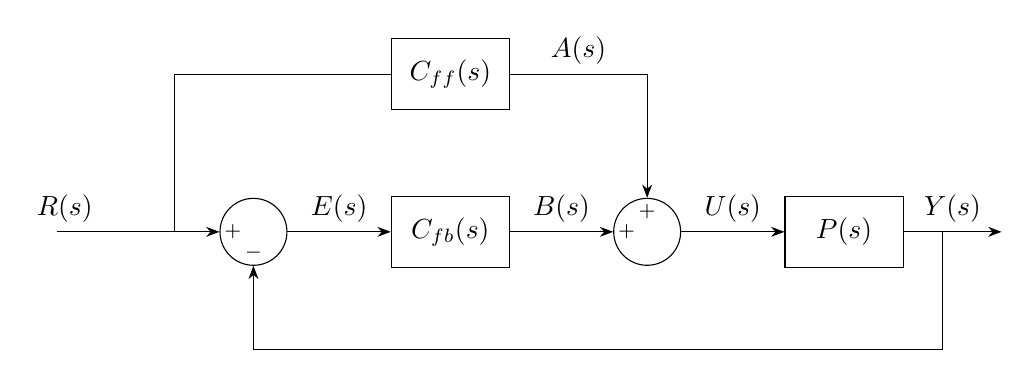
\begin{tikzpicture}[
    >=Stealth,
    block/.style={
        draw, rectangle,
        minimum width=1.5cm,
        minimum height=0.9cm
    },
    sum/.style={
        draw, circle,
        minimum size=0.85cm,
        inner sep=0pt
    }
]

    % Nodes
    \node[sum] (sum1) at (0,0) {};
    \node[block] (fb) at (2.5,0) {$C_{fb}(s)$};
    \node[block] (ff) at (2.5,2) {$C_{ff}(s)$};
    \node[sum] (sum2) at (5,0) {};
    \node[block] (plant) at (7.5,0) {$P(s)$};

    \coordinate (output) at (9.5,0);
    \coordinate (input) at (-2.5,0);
    \coordinate (branch) at (-1,0);

    % Reference input
    \draw[->] (input)
        -- node[pos=0.05,above] {$R(s)$} (sum1.west);

    % Feedforward branch
    \draw (branch) |- (ff.west);
    \draw[->] (ff.east) -| 
        node[pos=0.25,above] {$A(s)$} (sum2.north);

    % Feedback controller path
    \draw[->] (sum1.east)
        -- node[above] {$E(s)$} (fb.west);

    \draw[->] (fb.east)
        -- node[above] {$B(s)$} (sum2.west);

    % Plant input and output
    \draw[->] (sum2.east)
        -- node[above] {$U(s)$} (plant.west);

    \draw[->] (plant.east)
        -- node[above] {$Y(s)$} (output);

    % Negative feedback path
    \draw[->] (8.75,0) |- (0,-1.5) -| (sum1.south);

    % Summing junction signs
    \node at ($(sum1.west)+(0.17cm,0)$)
        {\scriptsize $+$};
    \node at ($(sum1.south)+(0,0.17cm)$)
        {\scriptsize $-$};

    \node at ($(sum2.west)+(0.17cm,0)$)
        {\scriptsize $+$};
    \node at ($(sum2.north)+(0,-0.17cm)$)
        {\scriptsize $+$};

\end{tikzpicture}
\end{center}

\tikzset{
    >=Stealth,
    block/.style={
        draw,
        rectangle,
        minimum width=1.55cm,
        minimum height=0.9cm
    },
    sum/.style={
        draw,
        circle,
        minimum size=0.55cm,
        inner sep=0pt
    }
}

%========================
% Series
%========================
\noindent\textbf{Series}

\begin{center}
\resizebox{\textwidth}{!}{
\begin{tikzpicture}[x=1cm,y=1cm]

% Original
\node (u1) at (0,0) {$U$};
\node[block] (g1) at (2,0) {$G_1$};
\node[block] (g2) at (4.4,0) {$G_2$};
\node (y1) at (6.4,0) {$Y$};

\draw[->] (u1) -- (g1.west);
\draw[->] (g1.east) -- (g2.west);
\draw[->] (g2.east) -- (y1);

\node at (7.7,0) {$\Longrightarrow$};

% Equivalent
\node (u2) at (9.3,0) {$U$};
\node[block, minimum width=2.2cm] (geq1)
    at (11.7,0) {$G_2G_1$};
\node (y2) at (13.9,0) {$Y$};

\draw[->] (u2) -- (geq1.west);
\draw[->] (geq1.east) -- (y2);

\end{tikzpicture}
}
\end{center}

%========================
% Parallel
%========================
\noindent\textbf{Parallel}

\begin{center}
\resizebox{\textwidth}{!}{
\begin{tikzpicture}[x=1cm,y=1cm]

% Original
\node (u3) at (0,0) {$U$};
\node[circle, fill, inner sep=1.6pt] (split) at (1.1,0) {};
\node[block] (pg1) at (3,0.85) {$G_1$};
\node[block] (pg2) at (3,-0.85) {$G_2$};
\node[sum] (psum) at (5.3,0) {};
\node (y3) at (6.7,0) {$Y$};

\draw[->] (u3) -- (split);
\draw (split.center) |- (pg1.west);
\draw (split.center) |- (pg2.west);
\draw[->] (pg1.east) -| (psum.north);
\draw[->] (pg2.east) -| (psum.south);
\draw[->] (psum.east) -- (y3);

% Summing junction signs
\node at ($(psum.north)+(0,-0.10)$) {\tiny $+$};
\node at ($(psum.south)+(0,0.10)$) {\tiny $+$};

\node at (8.0,0) {$\Longrightarrow$};

% Equivalent
\node (u4) at (9.6,0) {$U$};
\node[block, minimum width=2.4cm] (geq2)
    at (12.2,0) {$G_1+G_2$};
\node (y4) at (14.6,0) {$Y$};

\draw[->] (u4) -- (geq2.west);
\draw[->] (geq2.east) -- (y4);

\end{tikzpicture}
}
\end{center}

%========================
% Feedback
%========================
\noindent\textbf{Feedback}

\begin{center}
\resizebox{\textwidth}{!}{
\begin{tikzpicture}[x=1cm,y=1cm]

% Original
\node (u5) at (0,0) {$U$};
\node[sum] (fsum) at (1.1,0) {};
\node[block] (fg1) at (3,0) {$G_1$};
\node[circle, fill, inner sep=1.6pt] (pick) at (4.6,0) {};
\node (y5) at (5.8,0) {$Y$};
\node[block] (fg2) at (3,-1.45) {$G_2$};

\draw[->] (u5) -- (fsum.west);
\draw[->] (fsum.east)
    -- node[above] {$A$} (fg1.west);
\draw[->] (fg1.east) -- (pick.center);
\draw[->] (pick.center) -- (y5);

\draw[->] (pick.center) |- (fg2.east);
\draw[->] (fg2.west) -|
    node[pos=0.25,below] {$B$} (fsum.south);

% Summing junction signs
\node at ($(fsum.west)+(0.10,0)$) {\tiny $+$};
\node at ($(fsum.south)+(0,0.10)$) {\tiny $-$};

\node at (7.2,-0.05) {$\Longrightarrow$};

% Equivalent
\node (u6) at (8.9,0) {$U$};
\node[block, minimum width=3.0cm] (geq3)
    at (12.2,0) {$\dfrac{G_1}{1+G_1G_2}$};
\node (y6) at (15.0,0) {$Y$};

\draw[->] (u6) -- (geq3.west);
\draw[->] (geq3.east) -- (y6);

\end{tikzpicture}
}
\end{center}


\begin{center}
    {\Large\textbf{Block Diagram Transformation Rules}}
\end{center}

\tikzset{
    >=Stealth,
    block/.style={
        draw, rectangle,
        minimum width=1.15cm,
        minimum height=0.7cm,
        inner sep=2pt
    },
    sum/.style={
        draw, circle,
        minimum size=0.60cm,
        inner sep=0pt
    },
    junction/.style={
        circle, fill, inner sep=1.2pt
    }
}

%========================
% Rule 1
%========================
\noindent\textbf{Rule 1}

\begin{center}
\resizebox{\textwidth}{!}{
\begin{tikzpicture}

% Original
\node[sum] (s1) at (1,0) {};
\node[block] (g1) at (3,0) {$G$};

\draw[->] (0,0) -- (s1.west);
\draw[->] (s1.east) -- (g1.west);
\draw[->] (g1.east) -- (4.5,0);
\draw[->] (1,-1.4) -- (s1.south);

\node at ($(s1.west)+(0.16,0)$) {\tiny $\pm$};
\node at ($(s1.south)+(0,0.16)$) {\tiny $\pm$};

\node at (5.5,0) {$\Longleftrightarrow$};

% Equivalent
\node[block] (g2) at (7.5,0) {$G$};
\node[sum] (s2) at (9.5,0) {};
\node[block] (gb) at (9.5,-1.4) {$G$};

\draw[->] (6.2,0) -- (g2.west);
\draw[->] (g2.east) -- (s2.west);
\draw[->] (s2.east) -- (11,0);
\draw[->] (9.5,-2.4) -- (gb.south);
\draw[->] (gb.north) -- (s2.south);

\node at ($(s2.west)+(0.16,0)$) {\tiny $\pm$};
\node at ($(s2.south)+(0,0.16)$) {\tiny $\pm$};

\end{tikzpicture}
}
\end{center}

%========================
% Rule 2
%========================
\noindent\textbf{Rule 2}

\begin{center}
\resizebox{\textwidth}{!}{
\begin{tikzpicture}

% Original
\node[block] (g1) at (1.5,0) {$G$};
\node[sum] (s1) at (3.5,0) {};

\draw[->] (0,0) -- (g1.west);
\draw[->] (g1.east) -- (s1.west);
\draw[->] (s1.east) -- (5,0);
\draw[->] (3.5,-1.5) -- (s1.south);

\node at ($(s1.west)+(0.16,0)$) {\tiny $\pm$};
\node at ($(s1.south)+(0,0.16)$) {\tiny $\pm$};

\node at (6,0) {$\Longleftrightarrow$};

% Equivalent
\node[sum] (s2) at (7.8,0) {};
\node[block] (g2) at (9.8,0) {$G$};
\node[block] (inv) at (7.8,-1.5)
    {$\dfrac{1}{G}$};

\draw[->] (6.5,0) -- (s2.west);
\draw[->] (s2.east) -- (g2.west);
\draw[->] (g2.east) -- (11.3,0);
\draw[->] (7.8,-2.5) -- (inv.south);
\draw[->] (inv.north) -- (s2.south);

\node at ($(s2.west)+(0.16,0)$) {\tiny $\pm$};
\node at ($(s2.south)+(0,0.16)$) {\tiny $\pm$};

\end{tikzpicture}
}
\end{center}

%========================
% Rule 3
%========================
\noindent\textbf{Rule 3}

\begin{center}
\resizebox{\textwidth}{!}{
\begin{tikzpicture}

% Original
\node[block] (g1) at (1.5,0) {$G$};
\node[junction] (j1) at (3.2,0) {};

\draw[->] (0,0) -- (g1.west);
\draw[->] (g1.east) -- (4.8,0);
\draw[->] (j1.center) |- (4.8,-1);

\node at (5.8,0) {$\Longleftrightarrow$};

% Equivalent
\node[junction] (j2) at (7.2,0) {};
\node[block] (g2) at (9,0) {$G$};
\node[block] (g3) at (9,-1.3) {$G$};

\draw[->] (6.2,0) -- (j2.center);
\draw[->] (j2.center) -- (g2.west);
\draw[->] (g2.east) -- (11,0);
\draw[->] (j2.center) |- (g3.west);
\draw[->] (g3.east) -- (11,-1.3);

\end{tikzpicture}
}
\end{center}

%========================
% Rule 4
%========================
\noindent\textbf{Rule 4}

\begin{center}
\resizebox{\textwidth}{!}{
\begin{tikzpicture}

% Original
\node[junction] (j1) at (1,0) {};
\node[block] (g1) at (2.7,0) {$G$};

\draw[->] (0,0) -- (j1.center);
\draw[->] (j1.center) -- (g1.west);
\draw[->] (g1.east) -- (4.8,0);
\draw[->] (j1.center) |- (4.8,-1.3);

\node at (5.8,0) {$\Longleftrightarrow$};

% Equivalent
\node[block] (g2) at (7.8,0) {$G$};
\node[junction] (j2) at (9.7,0) {};
\node[block] (inv) at (10.6,-1.5)
    {$\dfrac{1}{G}$};

\draw[->] (6.3,0) -- (g2.west);
\draw[->] (g2.east) -- (j2.center);
\draw[->] (j2.center) -- (12.5,0);

% Branch moved downward with extra clearance
\draw[->] (j2.center) |- (inv.west);
\draw[->] (inv.east) -- (12.5,-1.5);

\end{tikzpicture}
}
\end{center}

%========================
% Rule 5
%========================
\noindent\textbf{Rule 5}

\begin{center}
\resizebox{\textwidth}{!}{
\begin{tikzpicture}

% Original feedback system
\node[sum] (s1) at (1.2,0) {};
\node[block] (g1) at (3.3,0) {$G$};
\node[junction] (j1) at (4.9,0) {};
\node[block] (h1) at (3.3,-1.5) {$H$};

% Reference input with label positioned away from junction
\draw[->] (-0.5,0)
    -- node[pos=0.18,above] {$R(s)$} (s1.west);

\draw[->] (s1.east) -- (g1.west);
\draw[->] (g1.east) -- (j1.center);
\draw[->] (j1.center)
    -- node[pos=0.8,above] {$Y(s)$} (6.3,0);

\draw[->] (j1.center) |- (h1.east);
\draw[->] (h1.west) -| (s1.south);

\node at ($(s1.west)+(0.16,0)$) {\tiny $\pm$};
\node at ($(s1.south)+(0,0.16)$) {\tiny $\pm$};

\node at (7.3,0) {$\Longleftrightarrow$};

% Equivalent feedback system
\node[block] (inv) at (9.8,0)
    {$\dfrac{1}{H}$};
\node[sum] (s2) at (12.1,0) {};
\node[block] (h2) at (14.3,0) {$H$};
\node[block] (g2) at (16.3,0) {$G$};
\node[junction] (j2) at (17.7,0) {};

% Extended reference line to prevent label overlap
\draw[->] (8.0,0)
    -- node[pos=0.18,above] {$R(s)$} (inv.west);

\draw[->] (inv.east) -- (s2.west);
\draw[->] (s2.east) -- (h2.west);
\draw[->] (h2.east) -- (g2.west);
\draw[->] (g2.east) -- (j2.center);

\draw[->] (j2.center)
    -- node[pos=0.8,above] {$Y(s)$} (19.2,0);

% Unity feedback
\draw[->] (j2.center) |- (12.1,-1.5) -- (s2.south);

\node at ($(s2.west)+(0.16,0)$) {\tiny $\pm$};
\node at ($(s2.south)+(0,0.16)$) {\tiny $\pm$};

\end{tikzpicture}
}
\end{center}




\end{document}
